\documentclass[12 pt, a4paper]{article}
\usepackage{amsmath, latexsym}
\usepackage{amsmath, amssymb}
\usepackage{amsopn}
\usepackage{float}
\usepackage{placeins}
\usepackage{mathrsfs}
\usepackage{amssymb}
\usepackage{enumerate}
\usepackage{paralist}
\usepackage{enumitem}
\usepackage{lipsum}
\usepackage{multirow}
\usepackage{multicol}
\usepackage[pdftex]{graphicx}
\usepackage[pdftex]{hyperref}
\usepackage{scalefnt}
\usepackage{setspace}
\usepackage{charter}
\usepackage{epsfig}
\usepackage{subfigure}
\usepackage{array,arydshln}
\usepackage{enumerate}
\usepackage{amsthm}
\usepackage{graphicx}
\usepackage{color,soul}
\usepackage{enumitem}
\usepackage{tcolorbox}
\usepackage{tikz}
\usetikzlibrary{arrows}
\usepackage{verbatim}
\usepackage{tabularx}
\usepackage[super]{nth}
\newtheorem{prop}{Proposition}
\newtheorem{thm}{Theorem}
\newtheorem{cor}[thm]{Corollary}
\newtheorem{lemma}[thm]{Lemma}
\newtheorem{remark}{Remark}
\usepackage{array}
\newtheorem{theorem}{Theorem}
%\theoremstyle{definition}
%\newtheorem{definition}{Definition}[section]
\newtheorem{definition}{Definition}
\usepackage{algorithm}
%\usepackage{algpseudocode}
\usepackage{algorithmic}
%%%%%%%%%%%%%%%%%%%%%%%%%%%%%%%%%%%%%%%
\usepackage{mathtools}
\usepackage{amsthm}
\usepackage{amsmath,amsfonts}
\usepackage{amssymb}
\usepackage[round]{natbib}
\setcitestyle{square}
\renewcommand{\sp}[1]{{ \text{Reg}(#1)}}
\def\I{{\mathcal I}}
\def\J{{\mathcal J}}
%\usepackage{stackengine}

%%%%%%%%%%%%%%%%%%%%%%%%%%%%%%%%%%%
\makeatletter
\def\BState{\State\hskip-\ALG@thistlm}
\makeatother

\newcommand{\HRule}{\rule{\linewidth}{1mm}}
\topmargin = -30 mm
\textwidth = 175 mm
\textheight = 270 mm
\oddsidemargin = -10 mm
\evensidemargin = -10 mm


\usepackage{listings}

\definecolor{dkgreen}{rgb}{0,0.6,0}
\definecolor{gray}{rgb}{0.5,0.5,0.5}
\definecolor{mauve}{rgb}{0.58,0,0.52}
\definecolor{codegreen}{rgb}{0,0.6,0}
\definecolor{codegray}{rgb}{0.5,0.5,0.5}
\definecolor{codepurple}{rgb}{0.58,0,0.82}
\definecolor{backcolour}{rgb}{1.00,1.00,1.00}

\lstdefinestyle{code}{language=Java,
  backgroundcolor=\color{backcolour},
  showstringspaces=false,
  columns=flexible,
  basicstyle={\ttfamily\footnotesize},
  numbers=left,
  numberstyle=\scriptsize\color{black},
  keywordstyle=\ttfamily\color{mauve},
  numbersep=5pt,
  commentstyle=\color{dkgreen},
  stringstyle=\color{mauve},
  breaklines=true,
  breakatwhitespace=false,
  tabsize=2,
  xleftmargin=1.0cm,
%  frame=bottomline,
  framexleftmargin=1.5em,
  framesep=2pt,
  escapechar=|,
}


%%%%%%%%%%%%%%%%%%%%%%%%%%%%%%%%%%% PAGE 1 %%%%%%%%%%%%%%%%%%%%%%%%%%%%%%%%%%%
\setlist[description]{font=\itshape}
\begin{document}
    \pagestyle{empty}
\vskip 0.2cm
	\begin{tabular}{p{4cm}p{11.5cm}}
		 \multirow{4}{*}{
\includegraphics[scale=0.25]{Images/Logo.jpg}} \\
		& \centering \large\bf\phantom{Empty line}\\ 
		\rule{0pt}{1pt} \centering \large\bf{INDIAN INSTITUTE OF TECHNOLOGY MANDI} \\
		\rule{0pt}{1pt} \centering \large\bf{HIMACHAL PRADESH, INDIA - 175075} \\
		\rule{0pt}{1pt} \centering \underline{\href{www.iitmandi.ac.in}{www.iitmandi.ac.in}}\\
	\end{tabular}
\noindent

{\raggedleft{}\HRule}
 
\begin{center}
\large\bf\underline{PROGRESS REPORT FOR THE ACADEMIC YEAR 2023}
\end{center}
\indent \textbf{Scholar's Name:} {ARJUN H KUMAR} \hfill \textbf{Roll No:} {S21008} \\
\noindent \textbf{School:} {SCEE} \hfill \textbf{Date of Registration: }{\nth{9} August 2021} \newline
\noindent \textbf{Semester:} {IV}\hfill \textbf{CGPA: }{8.57}
\newline
\noindent \textbf{Date of Last Presentation: }{\nth{29} July 2022}\hfill \textbf{Date of Current Presentation: }{x July 2023}
\\
\noindent\rule{17.69cm}{0.8pt}
   
\section{Research ~Objectives}
    
Using program analysis-
\begin{enumerate}
\item Identify various access patterns under which value-type objects should be flattened in their respective containers.
\item Build an appropriate flattening strategy for such objects in Eclipse OpenJ9 VM.
\item Improve Java applications by using a static + JIT analysis technique based on the developed flattening strategy.
\item Explore prospective optimizations that can be enabled in JVM due to the introduction of identity-less objects.

\end{enumerate} 

\section{Introduction}
In modern object-oriented programming languages, object identity
enables fundamental features such as field mutation and synchronization.
However, it also affects the performance and memory footprint of an application significantly. 
Each distinct field access requires a memory load of the corresponding object followed by an 
indirection to access the field object which is an additional overhead.
Moreover, every object is heap-allocated, and each heap-allocated object has headers of one or 
more words. An application may involve several 
thousand objects which contain such a predefined header. On the contrary, if an object is 
identity-less then the predefined header is no longer required and can contribute to reducing the 
memory footprint of the application.  Several compiler
analyses and optimizations such as escape analysis and field scalarization can eliminate 
these costs for the objects that maintain identity; however,
such optimizations are usually limited in their scope and applicability.


	Languages like Java allow for optimizing the access cost for
objects of certain “primitive” types, however object-oriented programs often
consist of user-defined types whose objects do not depend
on an identity that is separate from their value. An important
development in this space has been Project Valhalla \citep{PV}, which
aims to improve the performance profile of conventional objects in
Java, and make it comparable to the performance of primitive types.
Valhalla introduces the notion of value-types \citep{JEPD}, which essentially
empowers objects to be identity-less. To facilitate an improved 
performance for such objects, an important optimization
that can be performed by a value-types supporting Java Virtual
Machine (JVM) is object inlining or flattening \citep{ObjectInlining}.

\clearpage
%%%%%%%%%%%%%%%%%%%%%%%%%%%%%%%%%%% PAGE 1 END %%%%%%%%%%%%%%%%%%%%%%%%%%%%%%%%%%%

%%%%%%%%%%%%%%%%%%%%%%%%%%%%%%%%%%% PAGE 2 %%%%%%%%%%%%%%%%%%%%%%%%%%%%%%%%%%%
\setlist[description]{font=\itshape}
\pagestyle{empty}
\vskip 0.2cm
	\begin{tabular}{p{4cm}p{11.5cm}}
		 \multirow{4}{*}{
\includegraphics[scale=0.25]{Images/Logo.jpg}} \\
		& \centering \large\bf\phantom{Empty line}\\ 
		\rule{0pt}{1pt} \centering \large\bf{INDIAN INSTITUTE OF TECHNOLOGY MANDI} \\
		\rule{0pt}{1pt} \centering \large\bf{HIMACHAL PRADESH, INDIA - 175075} \\
		\rule{0pt}{1pt} \centering \underline{\href{www.iitmandi.ac.in}{www.iitmandi.ac.in}}\\
	\end{tabular}
\noindent

{\raggedleft{}\HRule}

\subsection{Object Flattening}
Flattening an object modifies the reference to a field inside a class object 
such that the object pointed to by the field is encoded directly inside the 
object of the class containing the same. This creates a compact memory representation
for the object containing the field.  
A flattened field inside an object avoids overheads from object headers, 
memory indirections, and heap allocation, and exhibits improved cache locality.
The object which contains the encoded
field object is termed the ``container'' object. 

Figure \ref{fig:Figure 1} illustrates the idea of flattening. 
Here, on the right-hand side, two {\em Point} objects, pointed to by 
the fields {\em start} and {\em end}, are inlined into a container object 
of type \textit{Line}.
As a result, accesses to the objects pointed to by {\em start} and {\em end} 
can be done directly from the container object of type {\em Line}. Moreover, 
the allocation costs and memory occupied for two {\em Point} objects are saved along
with a more coherent memory representation for {\em Line} object.

\begin{figure}[H]
	\vskip 0.2cm
	\centering
	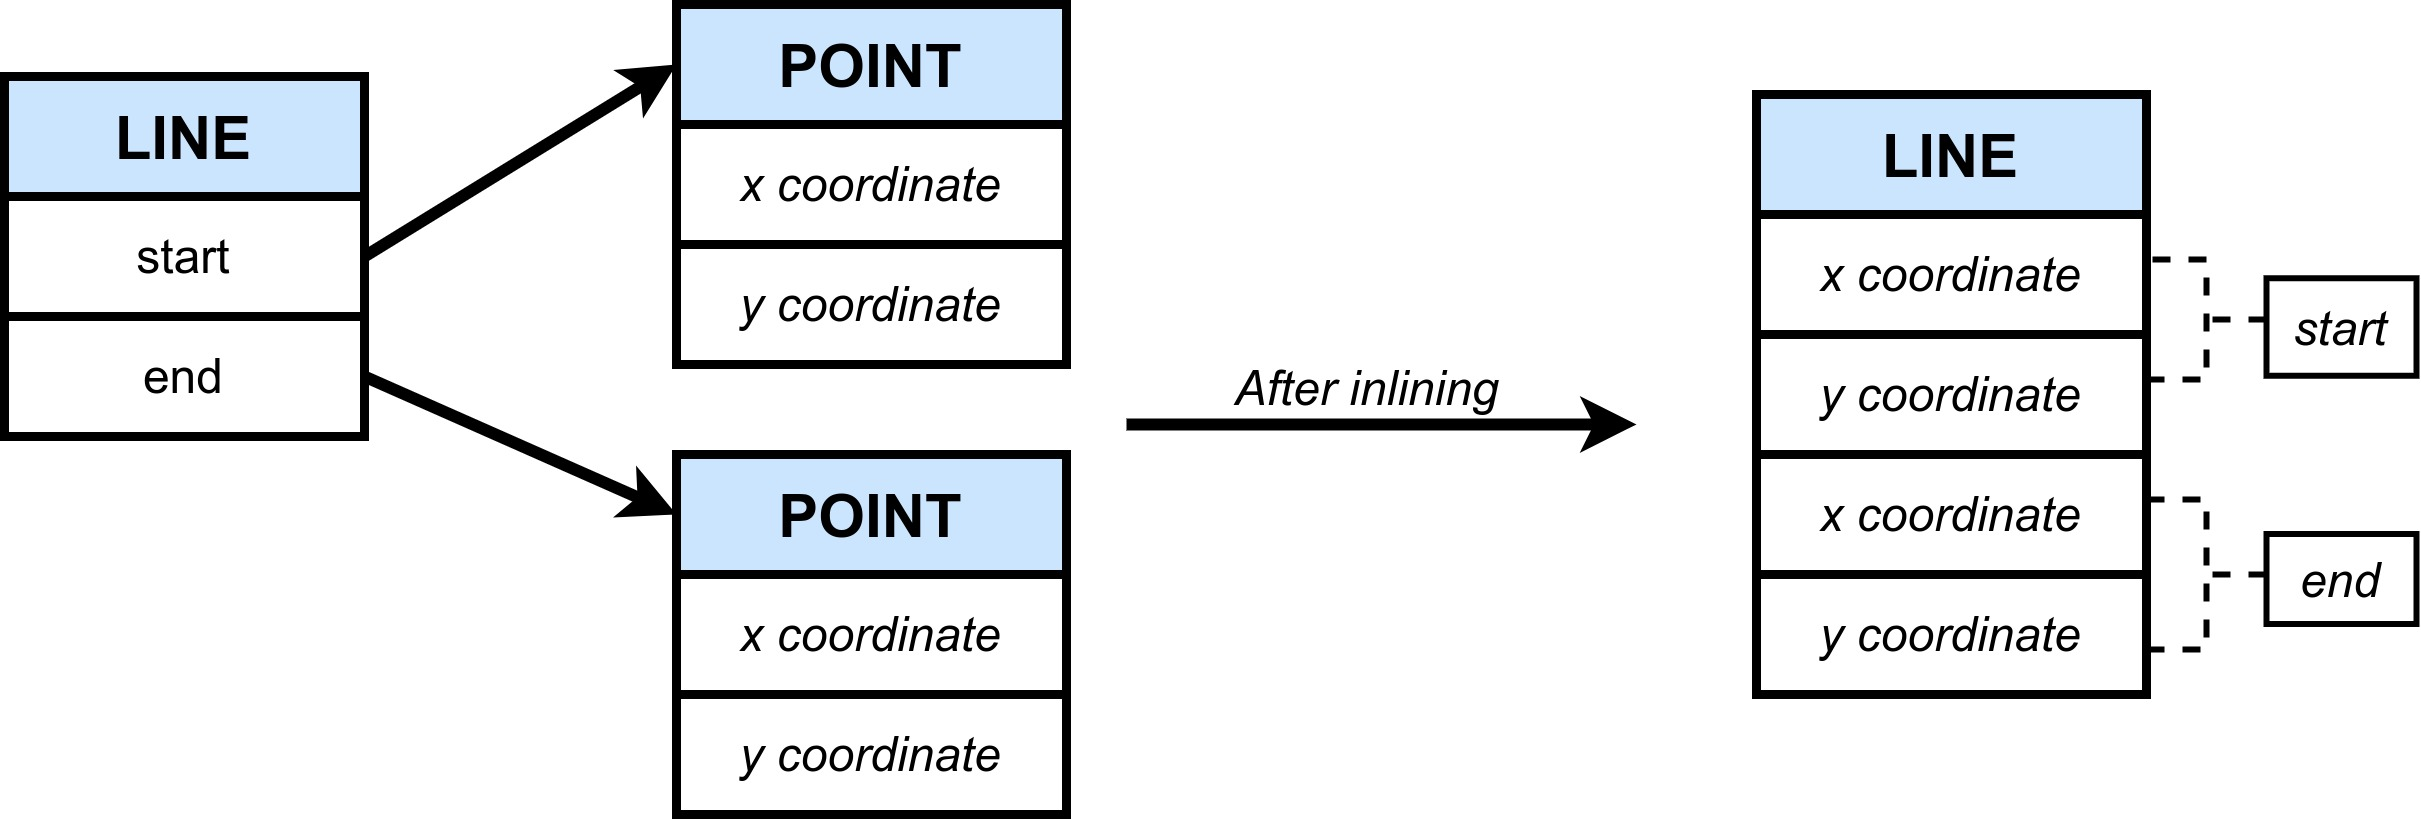
\includegraphics[scale=0.2]{Images/Flattening_Line.jpg}
	\caption{Flattening of objects}
	\label{fig:Figure 1}
\end{figure}
The flattening optimization needs to be performed carefully considering all the effects it can cause. 
For instance, flattening a field instance that is of large size or flattening too many objects into a 
container may lead to bloating. Bloating can impact the cache memory adversely and may 
lead to the potential loss of benefits gained by flattening. Another scenario is the case of object 
comparison in which a container object may suffer degradation in performance resulting 
from a high number of comparisons similar to the comparison operation performed by the native {\em String} class. 


	Such impactful factors may be determined by analyzing the source code statically in some cases, and in others may require 
information used during the execution of the program. Experimenting with programs that involve 
value-type objects and flattening optimization 
can help to discover more such impactful factors and access patterns to be considered for this 
optimization. 

Currently, in JVMs, a fixed parameter-based criterion is used to decide the flattening of objects.
Our research targets a combination of static + dynamic analyses, an idea from the PYE framework \citep{PYE2019} in 
order to selectively decide potential candidates for object flattening in the Eclipse OpenJ9 VM.
 We also intend to expand the optimizations 
possible in this VM in the context of value types. 

\clearpage
%%%%%%%%%%%%%%%%%%%%%%%%%%%%%%%%%%% PAGE 2 END %%%%%%%%%%%%%%%%%%%%%%%%%%%%%%%%%%%

%%%%%%%%%%%%%%%%%%%%%%%%%%%%%%%%%%% PAGE 3 %%%%%%%%%%%%%%%%%%%%%%%%%%%%%%%%%%%
\setlist[description]{font=\itshape}
\pagestyle{empty}
\vskip 0.2cm
	\begin{tabular}{p{4cm}p{11.5cm}}
		 \multirow{4}{*}{
\includegraphics[scale=0.25]{Images/Logo.jpg}} \\
		& \centering \large\bf\phantom{Empty line}\\ 
		\rule{0pt}{1pt} \centering \large\bf{INDIAN INSTITUTE OF TECHNOLOGY MANDI} \\
		\rule{0pt}{1pt} \centering \large\bf{HIMACHAL PRADESH, INDIA - 175075} \\
		\rule{0pt}{1pt} \centering \underline{\href{www.iitmandi.ac.in}{www.iitmandi.ac.in}}\\
	\end{tabular}
\noindent

{\raggedleft{}\HRule}

\section{Work Done and Target Set for Last Year}

\subsection{Study on implementation of object inlining inside the OpenJ9 VM}
\label{subsec:Subsection1}
It may neither be possible to inline all the objects of value-type classes (due to atomicity checks for 
nullness) nor may it be beneficial to do so.
Similar to the function of inlining optimization, inlining all potential candidates 
may lead to incoherently sized objects.
Imprudent increase in the size of objects may cause negative impacts on the memory efficiency of the 
corresponding application and may result 
in loss of all potential benefits obtained from object flattening. 


To ensure sanity and efficiency, the current implementation in Eclipse OpenJ9 \citep{OpenJ9} first filters value-type classes
by 
putting additional restrictions to identify primitive value-type classes, and then using a parameter-based strategy to 
limit the object size and decide if a field can be inlined into its corresponding container object. 
For this, a JVM parameter (-XX:ValueTypeFlatteningThreshold) has been introduced as a limiting
threshold. 
The parameter  specifies the maximum size (in bytes) of a 
flattenable object. 
Primitive value-type objects \citep{JEPP} that exceed this threshold size do not get 
optimized by flattening itself into its container instances. 
The instance size is computed dynamically considering all fields of an object 
and its predefined header size. The JVM parameter (-XX:ValueTypeFlatteningThreshold) is provided as input during runtime. 
By default the OpenJ9 VM 
considers this value to be {0} unless defined explicitly.
The workflow for the parameter-based strategy is described in Figure \ref{fig:Figure 2}.

\begin{figure}[h]
	\vskip 0.2cm
	\centering
	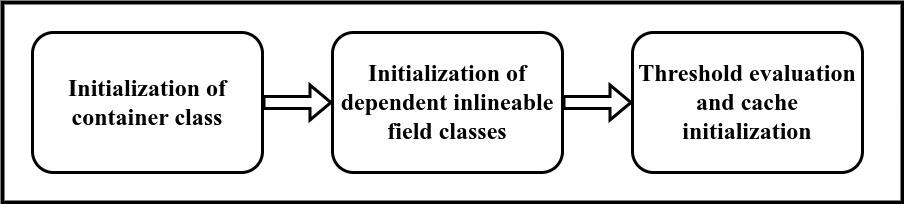
\includegraphics[scale=0.27]{Images/Class_Init.jpg}
	\caption{Flattening of objects}
	\label{fig:Figure 2}
\end{figure}



The bytecode `\textit{new}' resulting from the initialization of an object will trigger the loading 
of a class unless already done. 
During the initialization of a class, all the flattenable field value classes of the 
corresponding class are also loaded. This is done by analyzing the type-class descriptor.
Flattenable value classes have a unique type-class descriptor which is specifically prefixed 
with the character `\textit{Q}'. 
Once the flattenable field class has been loaded a threshold check is done. The Threshold 
condition is described in equation \ref{eq:equation1}.
\begin{equation}
	\label{eq:equation1}
	Instance Size \leq VM->Flattening Threshold
\end{equation} 

After the class loading of the value-type class is completed, the flattened field
cache for the corresponding container class is made an entry that describes the shape and modifiers 
of the flattened field. This field cache is used while instantiating
each instance of the class to track which fields are flattened.  
\clearpage
%%%%%%%%%%%%%%%%%%%%%%%%%%%%%%%%%%% PAGE 3 END %%%%%%%%%%%%%%%%%%%%%%%%%%%%%%%%%%%


%%%%%%%%%%%%%%%%%%%%%%%%%%%%%%%%%%% PAGE 4 %%%%%%%%%%%%%%%%%%%%%%%%%%%%%%%%%%%
\setlist[description]{font=\itshape}
\pagestyle{empty}
\vskip 0.2cm
	\begin{tabular}{p{4cm}p{11.5cm}}
		 \multirow{4}{*}{
\includegraphics[scale=0.25]{Images/Logo.jpg}} \\
		& \centering \large\bf\phantom{Empty line}\\ 
		\rule{0pt}{1pt} \centering \large\bf{INDIAN INSTITUTE OF TECHNOLOGY MANDI} \\
		\rule{0pt}{1pt} \centering \large\bf{HIMACHAL PRADESH, INDIA - 175075} \\
		\rule{0pt}{1pt} \centering \underline{\href{www.iitmandi.ac.in}{www.iitmandi.ac.in}}\\
	\end{tabular}
\noindent

{\raggedleft{}\HRule}

\subsection{Identification of value-type classes in programs}
Value-types although existed in OO languages like {\em C\#}; is a novel concept 
introduced for Java and is expected to be released as part of 
JDK-21. To experiment with such a cutting-edge feature 
codebases/ benchmarks needed to be explicitly created. 
As per the JEP specification \citep{JEPP} 
detailing the Flattened Heap Layouts for Value Objects,  
there exists a clear set of restrictions abiding which a class
can be flattened into their respective container class object.
A tool that can analyze existing codebases to find such classes which suffice the necessary conditions would help to
create a developmental space for experimenting with value-type objects and object flattening optimization.
 Motivated by this problem; a tool ``ValFinder'' was 
developed.
	
	

ValFinder uses the Soot framework \citep{soot} to perform static analysis
of Java Bytecode, and identifies classes that can be marked as value
and primitive. It then uses JavaParser \citep{JP} to transform Java source
code accordingly. ValFinder consists of two modules as described in Figure \ref{fig:Figure 3}.
\begin{enumerate}
	\item Analysis module
	\item Transformation module
\end{enumerate}


\begin{figure}[h]
	\vskip 0.2cm
	\centering
	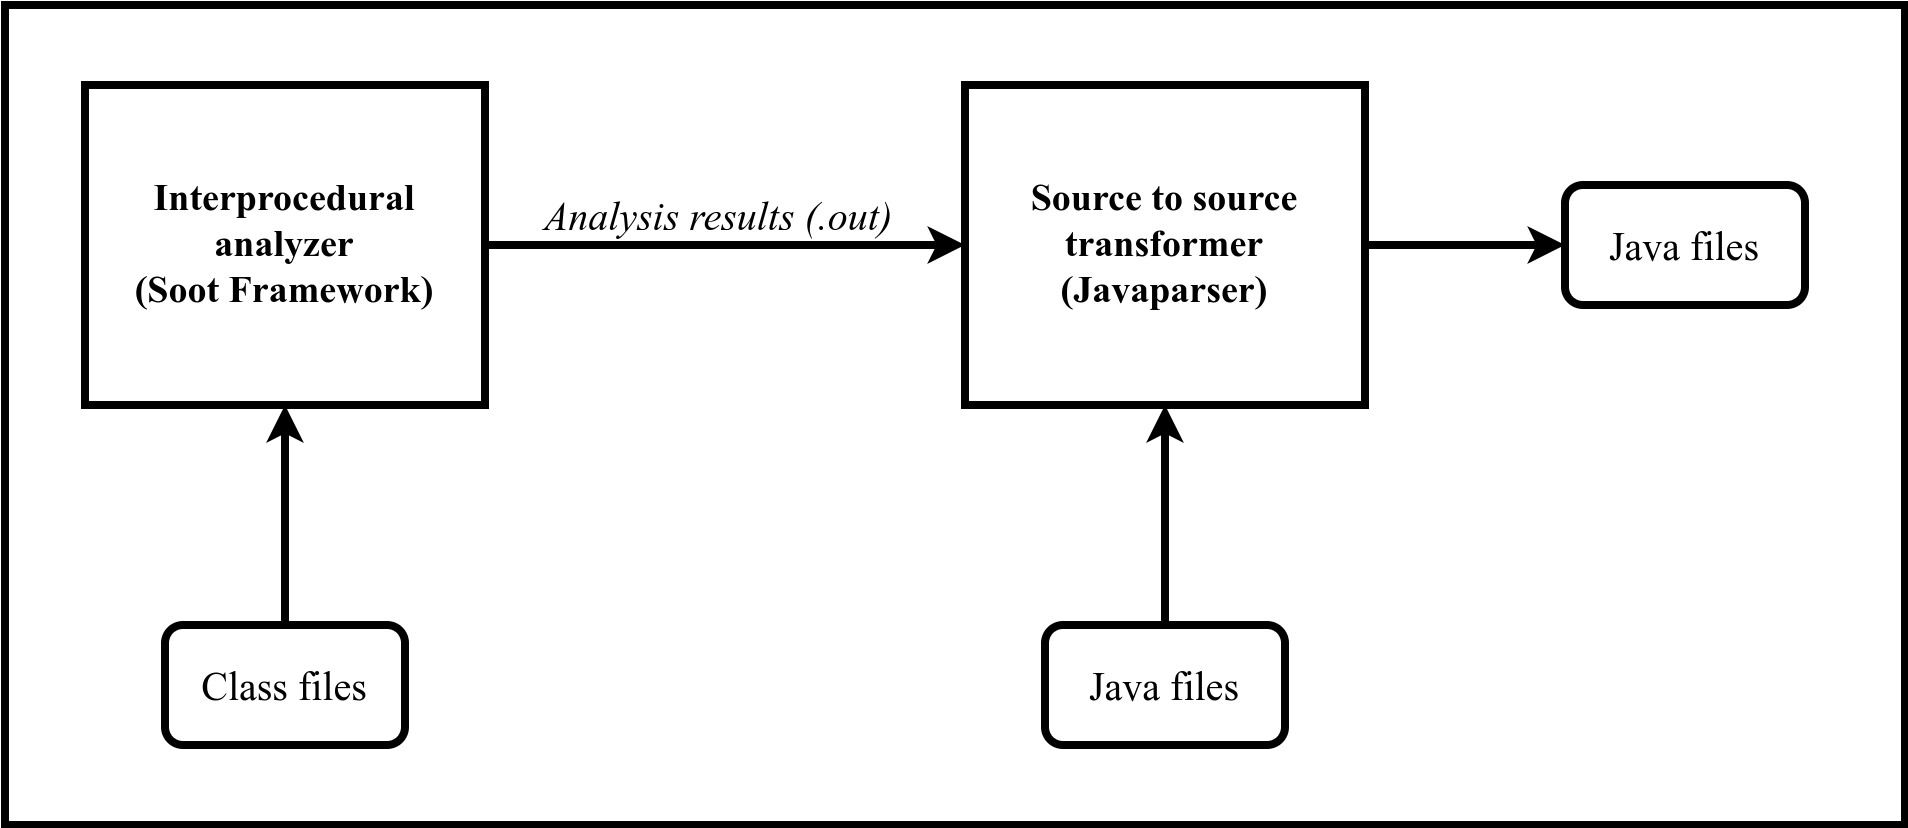
\includegraphics[scale=0.25]{Images/ValFinder.jpg}
	\caption{Overview of ValFinder}
	\label{fig:Figure 3}
\end{figure}


ValFinder starts by taking in the class files of a program that is to be analyzed as input and initiates performing an interprocedural
analysis from the analysis module.  In this module, the dependencies between various
classes and the value-type satisfiability conditions are evaluated. The output of this 
module is a subset of value and primitive classes identified from the input set. This subset of identified classes is fed to 
the transformation module along with the source code of the corresponding class files which were fed 
as input to the analysis module. In the transformation module, we use a modified JavaParser which supports 
the semantics of value-types classes. 

\clearpage
%%%%%%%%%%%%%%%%%%%%%%%%%%%%%%%%%%% PAGE 4 END %%%%%%%%%%%%%%%%%%%%%%%%%%%%%%%%%%%

%%%%%%%%%%%%%%%%%%%%%%%%%%%%%%%%%%% PAGE 5 %%%%%%%%%%%%%%%%%%%%%%%%%%%%%%%%%%%
\setlist[description]{font=\itshape}
\pagestyle{empty}
\vskip 0.2cm
	\begin{tabular}{p{4cm}p{11.5cm}}
		 \multirow{4}{*}{
\includegraphics[scale=0.25]{Images/Logo.jpg}} \\
		& \centering \large\bf\phantom{Empty line}\\ 
		\rule{0pt}{1pt} \centering \large\bf{INDIAN INSTITUTE OF TECHNOLOGY MANDI} \\
		\rule{0pt}{1pt} \centering \large\bf{HIMACHAL PRADESH, INDIA - 175075} \\
		\rule{0pt}{1pt} \centering \underline{\href{www.iitmandi.ac.in}{www.iitmandi.ac.in}}\\
	\end{tabular}
\noindent

{\raggedleft{}\HRule}

 Using the modified JavaParser we repair the source code of the classes identified 
during the analysis phase. 
This is achieved by iterating over the AST generated for the source code and subsequently modifying the node information. 
These changes are necessary so that the identified classes adhere to the syntactic specifications of 
value/primitive classes.
The output of this phase is hence the refactored source code which can potentially be benefitted through 
object flattening. This completes a pipeline for automatic source-to-source conversion of eligible non-value type classes 
to value-type classes.
ValFinder was further enhanced with various other auxiliary analyses to highlight the impact of restrictions that
cause non-compliance among classes.

\subsection{Granularity Change}
As per the JEP \citep{JEPP} specification and current implementation in JVMs, the instance size of a value-type object does not
change throughout the program execution. Hence when a value class is loaded for the first time, a flag is used to mark the class as flattenable or not.
Every instance field of a flattenable marked value-class type will get flattened irrespective of conditions other than the threshold size.
This level of granularity provides us with less control for flattening. There are instances of a value-type field that we
would prefer to inline and vice versa. To enable the same we modified the current implementation of Eclipse OpenJ9 VM to support field-level granularity over class-level granularity. 

For enabling field-level granularity; we need to pass information to the VM about which fields are to be considered for
flattening. This information is provided as input to the Eclipse OpenJ9 VM in the form of a {\em .out} file. This file contains a list 
of field metadata (field signature and corresponding container class signature). This information is sufficient to uniquely 
identify fields inside the VM.

For controlling the granularity level inside the VM; two new VM arguments have been introduced 
(-XX:+UseStaticResults and -XX:-UseStaticResults). -XX:+UseStaticResults flag 
instructs the VM to use field-level granularity and only consider the fields mentioned in the input {\em .out} file for flattening.
-XX:-UseStaticResults flag reverts the granularity to the class level where all eligible fields will get flattened.

During the VM initialization phase, the VM thread checks the granularity level based on the input parameters provided.
If the field-level granularity is specified then we read the '.out' file and store the corresponding field information in a 
global VM data structure. During the class initialization phase as described in section \ref{subsec:Subsection1}; we match the class signature of the
acting container class and iterate its fields to match the field signature from the global data structure.
Once the field has been identified as a potential flattening candidate we proceed with the threshold condition check and 
class cache initialization similar to native implementation described in section \ref{subsec:Subsection1}.

Along with a finer granularity level; the modifications to the Eclipse OpenJ9 VM align with our 
approach of using a static +  dynamic scheme to selectively flatten objects. By tuning the input {\em .out} 
file provided to the VM we can decide which fields are to be considered for flattening and vice versa.
% The next level of granularity to be considered is the object level.
This mechanism helps us to statically analyze code and pass insightful results to the JVM ecosystem where
 flattening decision is ultimately made. 


\clearpage


%%%%%%%%%%%%%%%%%%%%%%%%%%%%%%%%%%% PAGE 5 END %%%%%%%%%%%%%%%%%%%%%%%%%%%%%%%%%%%

%%%%%%%%%%%%%%%%%%%%%%%%%%%%%%%%%%% PAGE 6 %%%%%%%%%%%%%%%%%%%%%%%%%%%%%%%%%%%

\setlist[description]{font=\itshape}
\pagestyle{empty}
\vskip 0.2cm
	\begin{tabular}{p{4cm}p{11.5cm}}
		 \multirow{4}{*}{
\includegraphics[scale=0.25]{Images/Logo.jpg}} \\
		& \centering \large\bf\phantom{Empty line}\\ 
		\rule{0pt}{1pt} \centering \large\bf{INDIAN INSTITUTE OF TECHNOLOGY MANDI} \\
		\rule{0pt}{1pt} \centering \large\bf{HIMACHAL PRADESH, INDIA - 175075} \\
		\rule{0pt}{1pt} \centering \underline{\href{www.iitmandi.ac.in}{www.iitmandi.ac.in}}\\
	\end{tabular}
\noindent

{\raggedleft{}\HRule}
\section{Planned Work for the Next Year}   
 \begin{enumerate}
\item Implementing a static + dynamic analysis to compute the number of distinct
		cache loads possible between two inlined field loads.

\item Completing an end to end pipeline retrofitting all the analyses together.

\item Evaluating the strategy over a set of standard benchmarks for JVM.

\item Preparing a manuscript describing the complete work.
 
\end{enumerate} 





\vskip 0.7cm
\section{Workshops/Conferences Attended}
\begin{enumerate}
\item International Conference on Systems, Programming, 
Languages, and Applications: Software for Humanity 
(SPLASH Companion), Virtual, December 5th-10th, 2022.
\item \nth{16} Innovations in Software Engineering Conference (ISEC), 
IIIT Allahabad, India, February 23rd-25th, 2023.
\item Software Engineering Research in India (SERI) Update Meeting, 
Goa University, India, June 2nd-3rd, 2023
\end{enumerate} 



\section{Papers Published/Communicated and Other Achievements:} 
\begin{enumerate}
\item Arjun Harikumar and Manas Thakur. “ValFinder: Finding Hidden Value-Type Classes”. 
6th Workshop on Advances in Open Runtimes and Cloud Performance Technologies (AORCPT), part of IBM WeaveSphere, Toronto, Canada, November 16th, 2022.
\end{enumerate} 


\clearpage

%%%%%%%%%%%%%%%%%%%%%%%%%%%%%%%%%%% PAGE 6 END %%%%%%%%%%%%%%%%%%%%%%%%%%%%%%%%%%%

%%%%%%%%%%%%%%%%%%%%%%%%%%%%%%%%%%% PAGE 7 %%%%%%%%%%%%%%%%%%%%%%%%%%%%%%%%%%%

\setlist[description]{font=\itshape}
\pagestyle{empty}
\vskip 0.2cm
	\begin{tabular}{p{4cm}p{11.5cm}}
		 \multirow{4}{*}{
\includegraphics[scale=0.25]{Images/Logo.jpg}} \\
		& \centering \large\bf\phantom{Empty line}\\ 
		\rule{0pt}{1pt} \centering \large\bf{INDIAN INSTITUTE OF TECHNOLOGY MANDI} \\
		\rule{0pt}{1pt} \centering \large\bf{HIMACHAL PRADESH, INDIA - 175075} \\
		\rule{0pt}{1pt} \centering \underline{\href{www.iitmandi.ac.in}{www.iitmandi.ac.in}}\\
	\end{tabular}
\noindent

{\raggedleft{}\HRule}


\bibliographystyle{plainnat}
\bibliography{biblography}
     
\clearpage

%%%%%%%%%%%%%%%%%%%%%%%%%%%%%%%%%%% PAGE 6 END %%%%%%%%%%%%%%%%%%%%%%%%%%%%%%%%%%%


%%%%%%%%%%%%%%%%%%%%%%%%%%%%%%%%%%% PAGE 7 %%%%%%%%%%%%%%%%%%%%%%%%%%%%%%%%%%%

\setlist[description]{font=\itshape}

	\pagestyle{empty}
	\vskip 0.2cm
	\begin{tabular}{p{4cm}p{11.5cm}}
		 \multirow{4}{*}{
\includegraphics[scale=0.25]{Images/Logo.jpg}} \\
		& \centering \large\bf\phantom{Empty line}\\ 
		\rule{0pt}{1pt} \centering \large\bf{INDIAN INSTITUTE OF TECHNOLOGY MANDI} \\
		\rule{0pt}{1pt} \centering \large\bf{HIMACHAL PRADESH, INDIA - 175075} \\
		\rule{0pt}{1pt} \centering \underline{\href{www.iitmandi.ac.in}{www.iitmandi.ac.in}}\\
	\end{tabular}
\noindent

{\raggedleft{}\HRule}
	\begin{center}
	\large\bf{\underline{REPORT BY APC/DC COMMITTEE}} 
	\end{center}

\begin{enumerate}
    \item \textbf{Has the student met the targets set for last year?}
    \vskip 0.2cm
	\textbf{(a) Mention the Achieved Targets:}
	
	\begin{itemize}
	    \item 
	    \item 
	\end{itemize}
	\textbf{(b) If not what are the major reasons?}
	\vskip 0.2cm
	\hskip 0.7 cm N/A
	\vspace{0.2cm}
	\item \textbf{Is there a reasonable target set for next year? Give detailed plan.}
% 	\vspace*{1.0 cm}
	\begin{figure}[h]
    % \vskip 0.2cm
    \centering  
    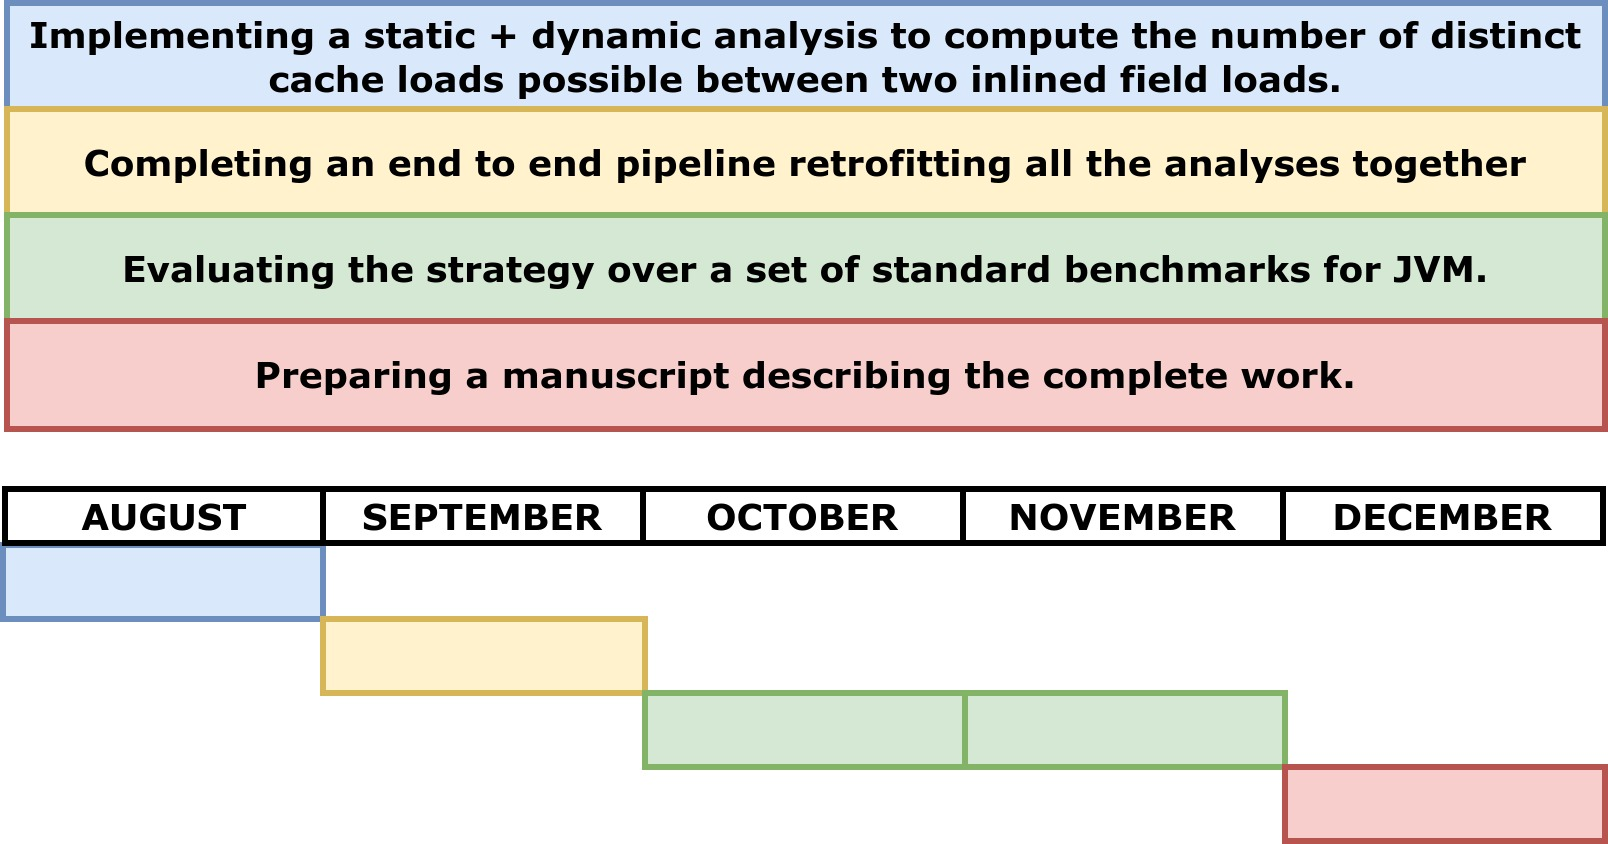
\includegraphics[scale=0.25]{Images/Gantt_Chart.jpg}
    \end{figure}
	\item \textbf{What is the perception of the student and guide(s) about the fraction of thesis work completed?}
	\vskip 0.2cm
	\hskip 0.7 cm \text{N/A}
	\item\textbf{What is the approximate time scale for thesis submission (only for students in their
		\bf \nth{5} year or above for Ph.D. and \nth{3} year and above for M.S. students).}
	\vskip 0.2cm
	\hskip 0.7 cm N/A
	\item\bf{Any other observations of the committee.}
	\vspace*{1.0 cm}


\end{enumerate}
\clearpage



%%%%%%%%%%%%%%%%%%%%%%%%%%%%%%%%%%% PAGE 7 END %%%%%%%%%%%%%%%%%%%%%%%%%%%%%%%%%%%


%%%%%%%%%%%%%%%%%%%%%%%%%%%%%%%%%%% PAGE 8 %%%%%%%%%%%%%%%%%%%%%%%%%%%%%%%%%%%



\setlist[description]{font=\itshape}
\pagestyle{empty}
\vskip 0.2cm
	\begin{tabular}{p{4cm}p{11.5cm}}
		 \multirow{4}{*}{
\includegraphics[scale=0.25]{Images/Logo.jpg}} \\
		& \centering \large\bf\phantom{Empty line}\\ 
		\rule{0pt}{1pt} \centering \large\bf{INDIAN INSTITUTE OF TECHNOLOGY MANDI} \\
		\rule{0pt}{1pt} \centering \large\bf{HIMACHAL PRADESH, INDIA - 175075} \\
		\rule{0pt}{1pt} \centering \underline{\href{www.iitmandi.ac.in}{www.iitmandi.ac.in}}\\
	\end{tabular}
\noindent

{\raggedleft{}\HRule}
\textbf{Recommendation of APC/DC} \textit{(Tick Appropriately)}
\begin{enumerate}
	\item
	\begin{enumerate}
\item Continuation of Registration is \textbf{Recommended/ Not Recommended.}
\item Continuation of Scholarship/Research Assistantship \textbf{ Recommended/ Not Recommended.}
\item Enhancement of Scholarship from JRF to SRF is \textbf{Recommended/ Not Recommended } (only
after Two Year of Registration).
\end{enumerate}
\item
\textbf{Source of Funding/Scholarship:}

\item \textbf{OVERALL PERFORMANCE: Very Good/Good/Satisfactory/Unsatisfactory}
\item \textbf{Any Other Recommendation/Comments} \textit{(Attach separate sheet).}
\end{enumerate}
\vspace*{0.5cm}

\noindent \textbf{COMMITTEE MEMBERS}\\\\
\indent
\begin{tabular}{|p{1.25cm}|p{5cm}|p{4cm}|p{3cm}|p{2cm}|}
	\hline\rule{0pt}{15pt} \bf S. No. & \bf Faculty Name & \bf School/Department & \bf Signature & \bf Remarks \\ 
	\hline\rule{0pt}{18pt}\bf 1. & Dr. A.D. Dileep  & SCEE &  &  \\[10pt]
	\hline\rule{0pt}{18pt}\bf 2. & Dr. Aditya Nigam & SCEE &  &  \\ [10pt]
	\hline \rule{0pt}{18pt}\bf3. & Dr. Gaurav Bhutani & SCEE &  &  \\ [10pt] 
	\hline \rule{0pt}{18pt}\bf4. & Dr. Manas Thakur & SCEE &  &  \\ [10pt] 
	\hline \rule{0pt}{18pt}\bf5. & Dr. Varunkumar Jayapaul & SCEE &  &  \\ [10pt]
	\hline 
\end{tabular} \\\\\\\\
\textbf{Signature of the Supervisor} \hspace{7.0cm} \textbf{School Chairperson}\\
Date: \hspace{11.3cm}  Date:\\
\vspace{1cm} \\
\hspace*{6cm}\textbf{Associate Dean (Research)}\\
\hspace*{6cm}Date:\\\\
\textbf{Note:}

\begin{enumerate}[label=(\roman*)]
	\item Ph.D. Scholar shall, after Registration, submit a written report to Doctoral Committee in the required
	format, annually for the first three years, and every six months thereafter.
	\item M.S. Scholar shall, after Registration, submit annually a written report to Academic Progress Committee.
	\item Attach additional sheets if required.
\end{enumerate}
\clearpage


%%%%%%%%%%%%%%%%%%%%%%%%%%%%%%%%%%% PAGE 8 END %%%%%%%%%%%%%%%%%%%%%%%%%%%%%%%%%%%


%%%%%%%%%%%%%%%%%%%%%%%%%%%%%%%%%%% PAGE 9 %%%%%%%%%%%%%%%%%%%%%%%%%%%%%%%%%%%
\setlist[description]{font=\itshape}
\pagestyle{empty}
\vskip 0.2cm
	\begin{tabular}{p{4cm}p{11.5cm}}
		 \multirow{4}{*}{
\includegraphics[scale=0.25]{Images/Logo.jpg}} \\
		& \centering \large\bf\phantom{Empty line}\\ 
		\rule{0pt}{1pt} \centering \large\bf{INDIAN INSTITUTE OF TECHNOLOGY MANDI} \\
		\rule{0pt}{1pt} \centering \large\bf{HIMACHAL PRADESH, INDIA - 175075} \\
		\rule{0pt}{1pt} \centering \underline{\href{www.iitmandi.ac.in}{www.iitmandi.ac.in}}\\
	\end{tabular}
\noindent

{\raggedleft{}\HRule}

\begin{center}
	\large\bf{\underline{APC/DC RECOMMENDATION (Part B)}} 
\end{center}


\noindent  \textbf{Scholar's Name:} {ARJUN H KUMAR} \hfill \textbf{Roll No:} {S21008} \\
\noindent \textbf{School:} {SCEE} \hfill \textbf{Date of APC/DC meeting: }{X July 2022}
\vskip 0.2cm
\noindent \begin{tabular}{|p{4.2cm}|p{5cm}|p{7cm}|}
\hline\rule{0pt}{7pt} \bf  & \centering \textbf{Performance} \centering \newline(Poor, Average, Good, Very good, Exceptional)  & \hspace{2.5cm}\bf Suggestions  \\[5pt] 
\hline\rule{0pt}{1pt} \begin{center} \bf Oral Communication and Presentation \end{center} &   &   \\[5pt]
\hline\rule{0pt}{1pt} \begin{center} \bf Subject Knowledge \end{center} &   &   \\[5pt]
\hline\rule{0pt}{1pt} \begin{center} \bf Research Output \end{center} &   &   \\[5pt]
\hline \multicolumn{3}{|c|}{{\multirow{1.5}{*}{ \textbf{OVERALL PERFORMANCE \textit{(as per Part-A): Very Good/Good/Satisfactory/Unsatisfactory:}}} 
} } \\
\multicolumn{3}{|c|}{}                  \\
\multicolumn{3}{|c|}{}                  \\

\hline \multicolumn{3}{|c|}{{\multirow{1.5}{*}{ \textbf{Overall feedback/Remarks:} } 
} } \\
\multicolumn{3}{|c|}{}                  \\
\multicolumn{3}{|c|}{}                  \\
\multicolumn{3}{|c|}{}                  \\
\hline 
\end{tabular} 
\vskip 0.4cm
\noindent \underline{\textbf{APC/Doctoral Committee}}
\vskip 0.3cm

\noindent\begin{tabular}{|p{4.5cm}|p{6cm}|p{4cm}|}
	\hline\rule{0pt}{15pt} \bf  & \bf Faculty Name & \bf Signature  \\ 
	\hline\rule{0pt}{18pt}\bf Chairperson APC/DC  & Dr. Aditya Nigam  &    \\[10pt]
	\hline\rule{0pt}{18pt}\bf Guide & Dr. Manas Thakur &   \\ [10pt]
	\hline \rule{0pt}{18pt}\bf Member  & Dr. A.D. Dileep &   \\ [10pt]
	\hline \rule{0pt}{18pt}\bf Member  & Dr. Gaurav Bhutani &   \\ [10pt] 
	\hline \rule{0pt}{18pt}\bf Member  & Dr. Varunkumar Jayapaul &   \\ [10pt] 
	\hline 
\end{tabular}


%%%%%%%%%%%%%%%%%%%%%%%%%%%%%%%%%%%%%%%
%\noindent \begin{tabular}{|p{4.2cm}|p{5cm}|p{7cm}|}
%\hline\rule{0pt}{5pt} \bf  & \begin{center} \textbf{Name of the Faculty} \end{center} &  \begin{center} \textbf{Signature} \end{center} \\[5pt] 
%\hline\rule{0pt}{18pt} \begin{center} \bf Chairperson APC/DC \end{center} &  \begin{center} Dr. Samar Agnihotri \end{center} &   \\[5pt]
%\hline\rule{0pt}{18pt} \begin{center} \bf Guide
 %\end{center} &  \begin{center} Dr. Manas Thakur \end{center} &   \\[5pt]
%\hline\rule{0pt}{18pt} \begin{center} \bf Co-Guide \end{center} &  \begin{center} \end{center} &   \\[5pt]
%\hline\rule{0pt}{18pt} \begin{center} \bf Member \end{center} &  \begin{center} Dr. Gaurav Bhutani \end{center} &   \\[5pt]
%\hline\rule{0pt}{18pt} \begin{center} \bf Member \end{center} &  \begin{center} Dr. Sriram Kailasam \end{center} &   \\[5pt]
%\hline
%\end{tabular}
%%%%%%%%%%%%%%%%%%%%%%%%%%%%%%%%%%%%%%%
\vskip 0.5cm
\noindent{I have read and noted the above for compliance.}
\vskip 0.2cm
\noindent\textbf{Signature of the scholar with Date:}

%%%%%%%%%%%%%%%%%%%%%%%%%%%%%%%%%%% PAGE 9 END %%%%%%%%%%%%%%%%%%%%%%%%%%%%%%%%%%%


\end{document}
